\documentclass{beamer}
\usetheme{Singapore}
\setbeamercovered{transparent}

\usepackage[english]{babel}
\usepackage[utf8]{inputenc}
\usepackage{times}
\usepackage[T1]{fontenc}
\usepackage{graphicx}

\title{Exploratory Data Analysis}
\date{\small MATH 252 Progress Presentation}
\institute{ Kathmandu University \\ Department of Computational Mathematics}
\author{Aayush Shrestha \and Anmol Jha}

\subject{Exploratory Data Analysis}

\begin{document}
	
	\begin{frame}
		\titlepage
	\end{frame}
	
	\begin{frame}{Outline}
		\begin{enumerate}
			\item Introduction
			\item Objective
			\item Progressed Work
			\item Work to Complete
		\end{enumerate}
	\end{frame}
	
	\section{Introduction}
	\begin{frame}{Exploratory Data Analysis}
		Exploratory Data Analysis (EDA) is a method of analyzing data using statistical summaries and graphical representations.\\

		EDA is a critical step in any Data Analysis or Data Science project as it provides a better understanding of data set variables and their relationships shows and what data can reveal beyond formal modeling or hypothesis testing tasks, and it.\\
		
		It aids in determining how to best manipulate data sources to obtain the answers required, making it easier for data scientists to discover patterns, detect anomalies, determine test hypotheses, and validate assumptions.
		
	\end{frame}
	
	\begin{frame}{Dashboard}
		Dashboard is basically a GUI for Data Visualization. A dashboard is a good choice if you need to summarize and present a lot of information on a single window.
		
		Dashboard is one of the major tool for presenting the data as it gives at-a-glance views of key performance indicators(KPI) relevant to a particular objective. 
		
		Dashboard helps Data Analysts and Data Scientists perform many data-related tasks, and also provides a visual aid for other stakeholders to understand data, and make accurate data-based decisions.
		
	\end{frame}
	
	\section{Objective}
	\begin{frame}{Goals For the project}
		\begin{itemize}
			\item Familiarity with data cleaning, feature extraction, and data conversion.
			
			\item Describing the data using statistical method such as mean, median, standard deviation, correlation and so on.
			
			\item Implementation of different plots in R
			
			\item Implementation of a dashboard .
			
			\item Understanding and explaining the trends and outliers in the data based on the domain.
			
		\end{itemize}
	\end{frame}
	
	\section{Progressed Work}
		\begin{frame}{Initial View}
			\begin{figure}
				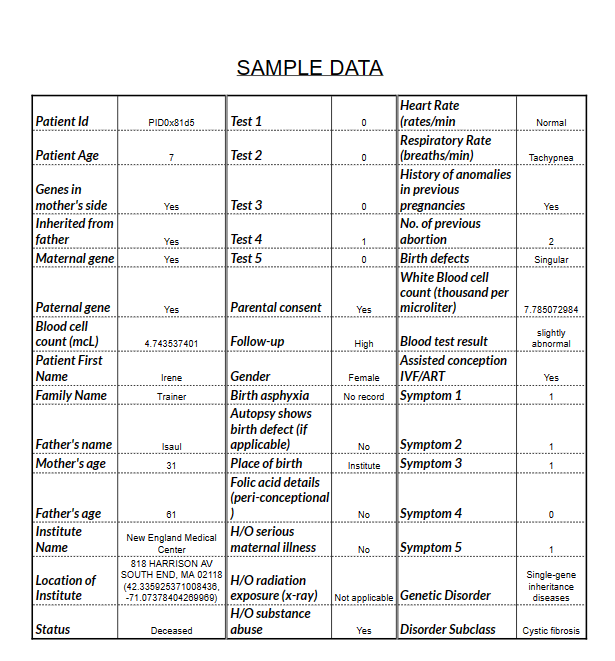
\includegraphics[width=0.65\textwidth, height=0.72\textheight]{sample.png}
				\caption{Sample raw data.}
			\end{figure}
		\end{frame}
		\begin{frame}{Removing Columns}
			The following Columns will not be useful in prediction of the disorder hence removed.\newline
			"Patient Id","Patient First Name","Family Name","Father's name","Institute Name","Location of Institute","Parental consent","Place of birth"\newline
			Below is the code:\newline
			\small{\textit{drop <- c("Patient Id","Patient First Name","Family Name","Father's name","Institute Name","Location of Institute","Parental consent","Place of birth")\newline
			df = df[,!(names(df) in drop)]}}
		\end{frame}
	\begin{frame}{Dashboard}
		% Content for the progressed dashboard work slide
	\end{frame}
	
	\section{Work to Complete}
	\begin{frame}{Exploratory Data Analysis}
		% Content for the work to complete in EDA slide
	\end{frame}
	
	\begin{frame}{Dashboard}
		% Content for the work to complete in the dashboard slide
	\end{frame}
	
\end{document}
